% =========================================================================
% CAPITOLO 1 — INTRODUZIONE
% =========================================================================

\chapter{Introduzione}
\label{ch:introduction}

\noindent
{\rmfamily\itshape
\begin{tabular}[t]{@{}l@{\hspace{0.3cm}}p{12.5cm}@{}}
\textls[50]{\textbf{Trattati:}} &
\textls[50]{Contesto e background · Allineamento con la missione personale ·
Tesi centrale · Posizionamento interdisciplinare · Rilevanza per l'innovazione e allineamento agli SDG}
\end{tabular}
}

\vspace{0.5cm}

Questo capitolo espone il problema che la tesi affronta, il vuoto che occupa, il caso di studio
attraverso cui lavora e la tesi che sostiene. Si chiude con una mappa dei capitoli che seguono.

% -------------------------------------------------------------------------
\section{Il problema: l'inaccessibilità cognitiva dei sistemi climatici complessi}
\label{sec:problem-of-knowing}

Per tre decenni la comunicazione del clima ha dato per scontato che le persone non agiscano perché mancano di informazioni, e che fatti migliori avrebbero colmato il divario. L'evidenza ha sistematicamente messo in discussione quest'idea. \citet{kellstedt2008} hanno rilevato che le persone che ne sapevano \emph{di più} sul cambiamento climatico riferivano spesso \emph{meno} preoccupazione e un più debole senso di responsabilità, anche controllando per orientamento politico e fattori demografici. \citet{kahan2015} ha mostrato che l'alfabetizzazione scientifica può ampliare anziché ridurre il disaccordo: le persone più competenti su fronti opposti divergono di più quando leggono le stesse evidenze. L'informazione, si scopre, è filtrata attraverso convinzioni pregresse, identità culturale e i meccanismi della cognizione. Il compito non è solo enunciare la scienza del clima in modo più accurato, ma presentarla in una forma che si accordi con il modo in cui le persone le danno effettivamente senso.

Un ostacolo più profondo sta sotto questo e precede il dibattito sul clima. In due decenni di esperimenti, \citet{sterman2008} ha rilevato che perfino persone molto istruite --- dottorandi del MIT, ingegneri, partecipanti con formazione matematica --- ragionano male sui sistemi fondati su accumulo e flusso. \citet{cronin2009} lo ha mostrato con chiarezza: dati il flusso in entrata e in uscita di un sistema e chiesto di tracciare lo stock accumulato, molti hanno confuso i tassi con i livelli e trattato un processo dinamico come statico. Non erano persone a cui mancava la matematica; la possedevano, e la rappresentazione statica le ha comunque sconfitte. L'implicazione per il clima è diretta: mostrare le emissioni di CO\textsubscript{2} e la concentrazione come due curve non trasmette che la seconda accumula la prima, per cui il pubblico sottostima l'inerzia che il sistema porta con sé \citep{cronin2009, sterman2008}. La teoria del carico cognitivo spiega perché: la memoria di lavoro è limitata, e una rappresentazione che chiede all'osservatore di animare mentalmente un processo nascosto impone un onere che cresce con la complessità del sistema \citep{sweller1988}.

Queste due letterature --- come viene interpretata l'informazione sul clima, e come le persone ragionano sui sistemi dinamici --- convergono su una sola conclusione. Comunicare un sistema climatico complesso non è principalmente un problema di accuratezza o di messaggio. È un problema di \emph{rappresentazione}: trovare forme in cui il comportamento dinamico, multiscala e potenzialmente non lineare di un tale sistema diventi qualcosa che una persona può percepire, anziché qualcosa che deve ricostruire nella propria mente a partire da un'immagine statica.


% -------------------------------------------------------------------------
\section{Il vuoto e la proposta}
\label{sec:gap-proposal}

Questo problema di rappresentazione è stato affrontato da due direzioni, ciascuna solida di per sé e raramente congiunte. La ricerca sulla visualizzazione del clima ha documentato in dettaglio perché i formati convenzionali falliscono con il pubblico non specialista --- e ha mostrato che le visualizzazioni che le persone trovano più chiare spesso non sono quelle che comprendono meglio \parencite{harold2016, hegarty2012}. Separatamente, il machine learning per la scienza del clima è cresciuto rapidamente, ma quasi interamente in un ruolo \emph{predittivo}: previsione, rilevamento di anomalie, miglioramento dei modelli per utenti esperti \citep{reichstein2019, sonnewald2021}. Ciò che si è quasi mai tentato è usare il machine learning non per predire, ma per \emph{recuperare la struttura nascosta} di un sistema climatico e trasformarla in una forma che i non specialisti possano percepire. Il vuoto che questa tesi occupa è l'intersezione dei due: la potenza analitica del secondo, rivolta al problema di rappresentazione nominato dal primo.\footnote{Entrambe le letterature sono esaminate per esteso nel Capitolo~\ref{ch:literature}, che colloca la tesi con precisione rispetto alla ricerca esistente sulla visualizzazione, alle applicazioni del machine learning e ai principi delle scienze cognitive che fondano il design.}

La tesi avanza quindi un'unica affermazione: che la struttura latente che un modello di machine learning recupera da un sistema climatico complesso può fungere da substrato per rappresentazioni che rendono quel sistema percepibile ai non specialisti --- e che se ciò accada debba essere stabilito per confronto con l'idioma convenzionale, non asserito. Per perseguirla, la tesi propone un \emph{framework integrativo} costruito in tre fasi, ciascuna delle quali attinge a una tradizione diversa e alimenta la successiva. La prima è \emph{analitica}: il machine learning non supervisionato è applicato a dati osservativi e di rianalisi, non per prevedere, ma per recuperare la struttura latente del sistema --- un insieme compatto di coordinate che ne cattura la dinamica essenziale (Capitolo~\ref{ch:data_pipeline}). La seconda è \emph{progettuale}: quelle strutture latenti sono tradotte in rappresentazioni esperienziali, con ogni scelta di design fondata su principi delle scienze cognitive, della cognizione incarnata e della visualizzazione delle informazioni (Capitolo~\ref{ch:translate}). La terza è \emph{empirica}: le rappresentazioni risultanti sono valutate rispetto a una baseline statica convenzionale attraverso uno studio con utenti a metodi misti, verificando se cambino il modo in cui il pubblico non specialista comprende il sistema (Capitolo~\ref{ch:userstudy}).
% -------------------------------------------------------------------------
\section{Il caso di studio: l'AMOC come banco di prova del framework}
\label{sec:case-study-amoc}

Un framework come questo ha bisogno di un caso abbastanza impegnativo da metterlo alla prova, che porti con sé proprio le caratteristiche che rendono difficile la comunicazione.\footnote{L'AMOC è usata solo come caso di prova. Questa tesi non avanza alcuna nuova affermazione oceanografica e non contribuisce alla ricerca sulla circolazione oceanica; si occupa dell'AMOC unicamente attraverso gli aspetti rilevanti per il problema di rappresentazione. Le sue basi fisiche sono esposte nel Capitolo~\ref{ch:background}.} La Atlantic Meridional Overturning Circulation (AMOC) è un sistema di questo tipo. È invisibile in senso forte: nessuna manifestazione superficiale la rivela, e nessuna esperienza quotidiana vi dà accesso. Si estende su un bacino oceanico, per cui nessun singolo punto ne mostra il comportamento, e varia su scale da decenni a secoli --- più lunghe sia dell'esperienza umana sia del record osservativo. È non lineare ed è un candidato elemento di tipping, il cui indebolimento sostanziale potrebbe spostare la circolazione in un regime diverso con isteresi \citep{armstrongmckay2022, lenton2008}, riorganizzando il trasporto di calore del Nord Atlantico e ridisegnando il clima d'Europa \citep{buckley2016}. La sua intensità si misura in sverdrup (Sv) ed è osservata con continuità dal 2004 dall'array RAPID a \ang{26.5}~nord \citep{frajkawilliams2021, moat2026}, con il Copernicus Global Reanalysis Ensemble Product (GREP) che ne estende il record più indietro nel tempo.

L'AMOC non è il sistema che la maggior parte delle persone immagina pensando al cambiamento climatico: a chi deve immaginarla, i non specialisti nominano cose visibili --- ghiaccio che si scioglie, caldo estremo, mari che si alzano \citep{oneill2014}. Quel contrasto, tra i sistemi climatici che possiamo vedere e quelli che richiedono strumenti e calcolo anche solo per essere percepiti, è centrale nell'argomentazione qui, e i due non sono indipendenti. La calotta glaciale della Groenlandia, tra i segni più visibili di un mondo che si riscalda, è fisicamente accoppiata all'AMOC: l'acqua dolce dalla Groenlandia abbassa la densità dell'acqua superficiale del Nord Atlantico, indebolisce la formazione di acque profonde e può rallentare la circolazione \citep{boning2016, caesar2018, rahmstorf2015}. Questa tesi usa quel ponte, dal ghiacciaio visibile alla corrente nascosta, come punto d'ingresso nel sistema invisibile.\footnote{Il comportamento recente dell'AMOC è esso stesso oggetto di dibattito: alcune ricostruzioni suggeriscono un indebolimento di lungo periodo e un possibile avvicinamento a una transizione \citep{caesar2018, boers2021, ditlevsen2023}, lettura contestata su basi metodologiche \citep{benyami2024}, mentre il record diretto RAPID non mostra un chiaro rallentamento di lungo periodo \citep{moat2026}. Questo dibattito irrisolto rende una rappresentazione chiara più necessaria, non meno.}

% -------------------------------------------------------------------------
\section{Sulla natura interdisciplinare del lavoro}
\label{sec:positioning}

Ho iniziato questo lavoro spinto da una missione personale: \emph{Wisdom Unlocks Awareness, and Awareness Unlocks Agency}. La comprensione è ciò che dà alla conoscenza il potere di muovere le persone --- non solo a sapere, ma a tenerci, e poi ad agire. Le persone raramente agiscono perché viene detto loro che un sistema conta; agiscono una volta che lo colgono.

Questa tesi si colloca dove si incontrano cinque discipline. La \emph{scienza del clima} fornisce il sistema, i dati e gli standard di evidenza. Il \emph{machine learning} recupera struttura nascosta da dati troppo ad alta dimensionalità per l'occhio --- e qui sta per una convinzione più ampia, che le tecnologie emergenti usate per le persone possano essere strumenti di comprensione, non solo motori di previsione. Le \emph{scienze cognitive} spiegano perché i sistemi dinamici sconfiggono l'intuizione. La \emph{visualizzazione delle informazioni} fornisce i principi per trasformare la struttura in qualcosa che l'occhio possa leggere. E la \emph{comunicazione della scienza} pone la prova finale: non se una rappresentazione sia accurata, ma se un non specialista ne esca avendo capito.

Il contributo non risiede in nessuno di questi campi da solo, ma nel legarli insieme. L'evidenza, il calcolo che la rivela e la forma in cui una persona infine la incontra sono di solito trattati separatamente, da persone diverse, in letterature diverse. Questa tesi li mette in un'unica catena --- perché ciò su cui una società può agire è limitato da ciò che può prima comprendere.\footnote{Questa sezione enuncia la posizione da cui il lavoro è stato intrapreso. L'evidenza per ciascuna delle affermazioni che raccoglie è presentata nel Capitolo~\ref{ch:literature}.}

% -------------------------------------------------------------------------
\section{Contributo, rilevanza per l'innovazione e allineamento agli SDG}
\label{sec:contribution}

Il contributo è principalmente metodologico: non un nuovo risultato sull'oceano o una nuova tecnica di machine learning, ma un modo di unire due cose di solito tenute separate --- ciò che l'analisi rivela su un sistema climatico complesso, e la forma percettiva in cui un non specialista lo incontra. Poiché è verificato rispetto a una baseline convenzionale anziché presentato da solo, il suo valore poggia sull'evidenza anziché sull'asserzione. Rispetto al lavoro esistente è distintivo nel combinare quattro elementi non prima riuniti: recuperare la struttura latente di un sistema di tipping tramite machine learning, tradurla in una rappresentazione esperienziale, fondare ciascuna scelta su principi delle scienze cognitive e valutare il risultato in modo comparativo.\footnote{Quattro famiglie di lavori correlati --- visualizzazione statica convenzionale, strumenti climatici interattivi, formati immersivi ed esperienziali, e physicalisation dei dati --- sono esaminate nel Capitolo~\ref{ch:literature}. Nessuna integra tutti e quattro gli elementi sopra.}

La rilevanza si articola su tre livelli. \emph{Accademicamente}, la ricerca sulla comunicazione dei sistemi climatici complessi si è appoggiata agli studi di preferenza più che alla comprensione verificata, e i formati esperienziali restano in gran parte non valutati; questa tesi offre una metodologia comparativa anziché un'altra visualizzazione. \emph{Istituzionalmente}, si allinea in modo sostanziale agli Obiettivi di Sviluppo Sostenibile delle Nazioni Unite: in primo luogo \textbf{SDG~13 (Lotta al cambiamento climatico)}, target~13.3 su educazione, consapevolezza e capacità \citep{un2015}; in secondo luogo \textbf{SDG~4 (Istruzione di qualità)}, nel rendere accessibile una scienza complessa; e indirettamente \textbf{SDG~14 (La vita sott'acqua)}, poiché l'AMOC fa parte del sistema oceanico. \emph{Praticamente}, il framework è costruito per trasferirsi: l'AMOC è uno di una famiglia di elementi di tipping --- calotte glaciali, l'Amazzonia, il permafrost, il monsone --- che condividono invisibilità, lunghe scale temporali, non linearità e alta posta in gioco \citep{armstrongmckay2022, lenton2008}. Prima che una società possa agire su un sistema complesso, deve prima essere in grado di raffigurarselo; questa tesi è un contributo a imparare come.

% it/figures/sdg/sdg_alignment.tex — versione italiana
\begin{figure}[!ht]
    \centering
    
\includegraphics[height=4cm]{figures/sdg/sdg4.png}\hfill
    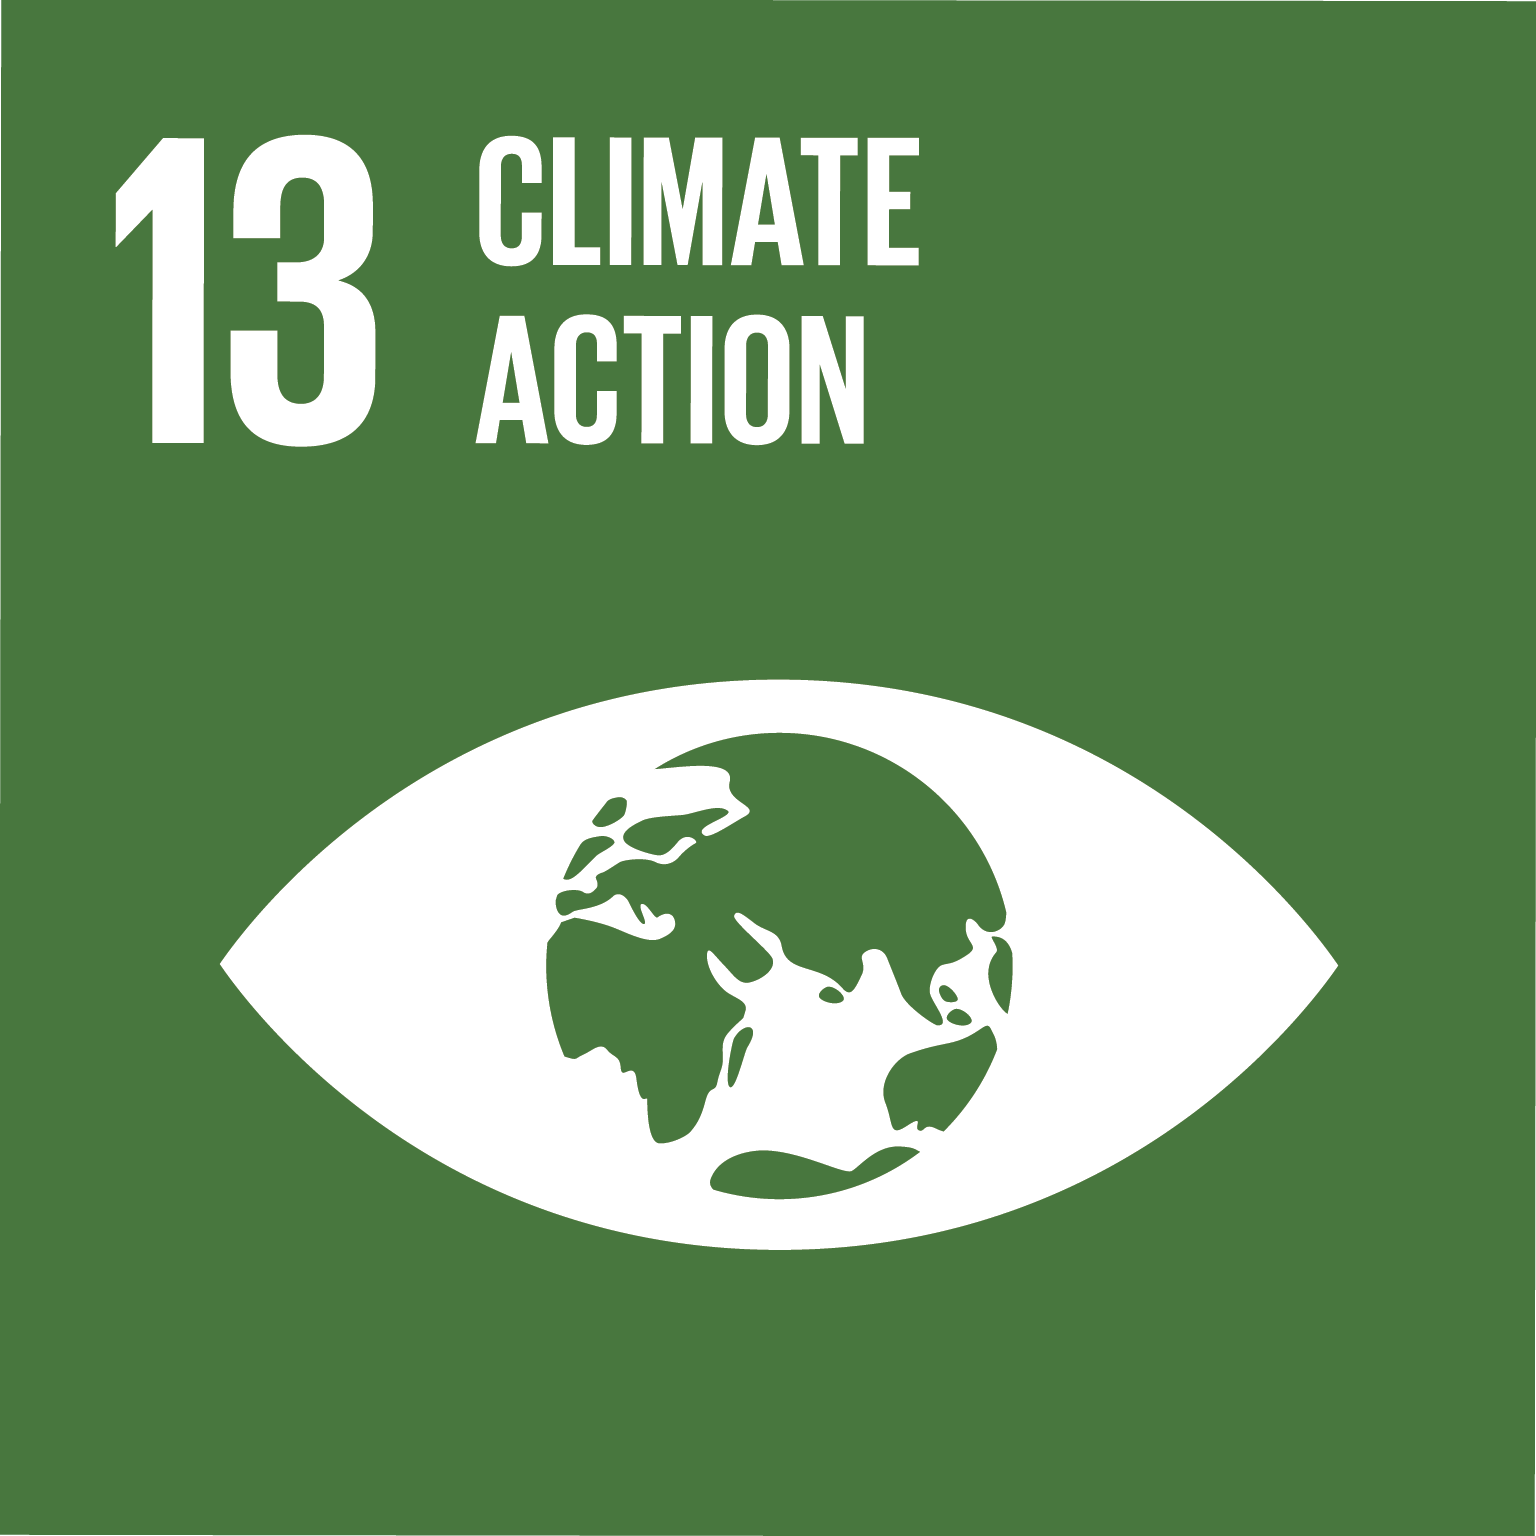
\includegraphics[height=4cm]{figures/sdg/sdg13.png}\hfill
    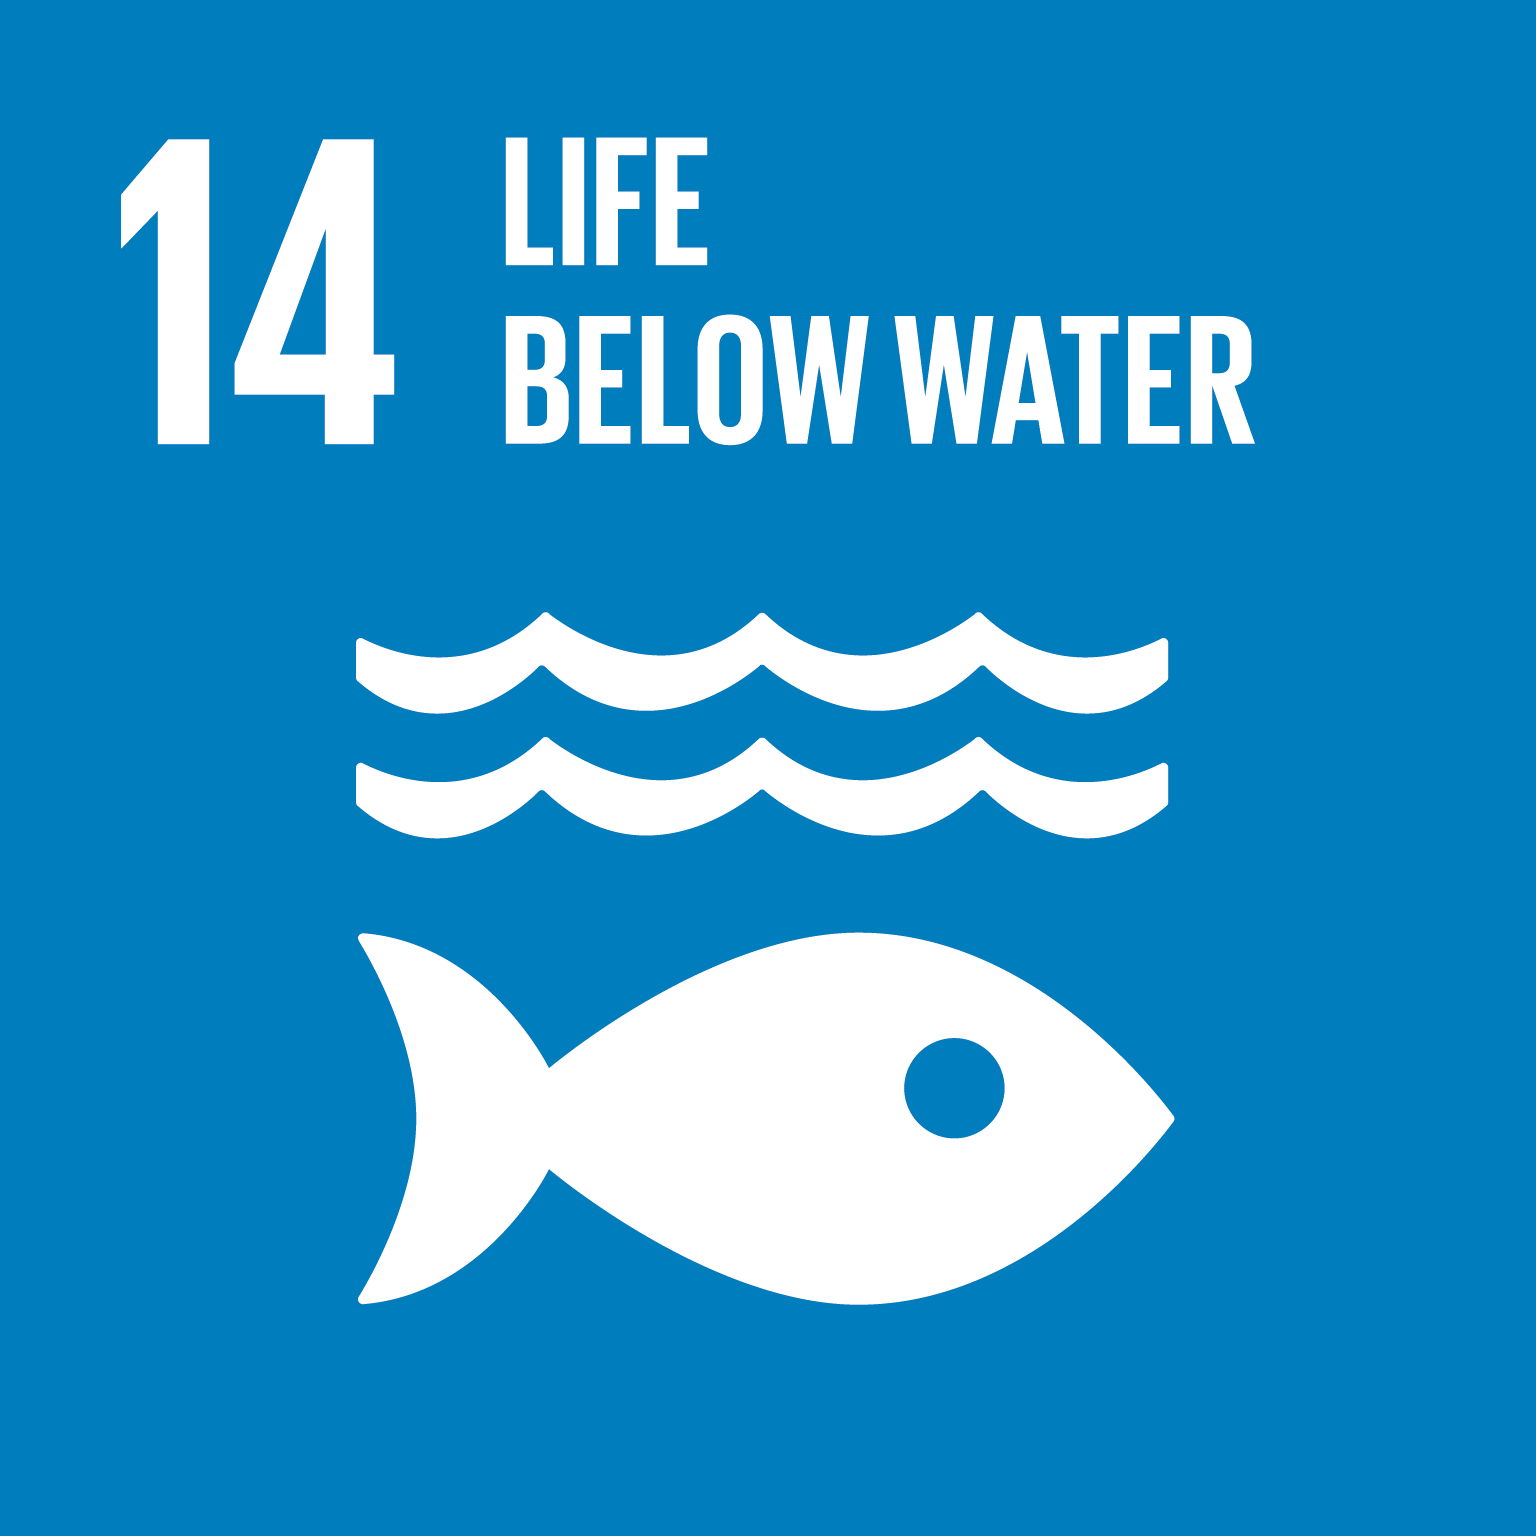
\includegraphics[height=4cm]{figures/sdg/sdg14.png}
    \caption[Obiettivi di Sviluppo Sostenibile affrontati da questa tesi.]{\textbf{I
    tre Obiettivi di Sviluppo Sostenibile a cui questa tesi contribuisce.} SDG~13
    (Lotta al cambiamento climatico), in particolare il target~13.3 su educazione,
    consapevolezza e capacità; SDG~4 (Istruzione di qualità), sul rendere accessibile
    la conoscenza complessa; e SDG~14 (La vita sott'acqua), poiché l'AMOC fa parte del
    sistema oceanico. Icone \textcopyright~Nazioni Unite. Il contenuto di questa
    pubblicazione non è stato approvato dalle Nazioni Unite e non ne riflette le
    opinioni.}
    \label{fig:sdg-alignment}
\end{figure}


% -------------------------------------------------------------------------
\section{Mappa della tesi}
\label{sec:roadmap}

La tesi è organizzata attorno all'arco rilevare--tradurre--valutare, in tre parti.

\textbf{Parte~I --- RILEVARE} imposta il problema e fornisce la base analitica su cui costruisce il resto della tesi. Il Capitolo~\ref{ch:rqs} formalizza le domande di ricerca, gli obiettivi, le ipotesi e le proposizioni progettuali. Il Capitolo~\ref{ch:literature} esamina la letteratura, vi colloca la tesi e deriva la grammatica di design che in seguito governa ogni scelta di rappresentazione. Il Capitolo~\ref{ch:background} sviluppa l'apparato fisico e matematico necessario a trattare l'AMOC come oggetto analizzabile. Il Capitolo~\ref{ch:methodology} specifica la metodologia che governa tutte e tre le fasi e lo standard di evidenza a cui ciascuna risponde. Il Capitolo~\ref{ch:data_pipeline} svolge poi l'analisi vera e propria, riducendo la struttura verticale dell'AMOC a uno spazio latente compatto e interpretabile, verificando se quella riduzione sia fedele e caratterizzando le anomalie del record e il suo comportamento di preallarme.

\textbf{Parte~II --- TRADURRE} documenta il lavoro costruttivo. Il Capitolo~\ref{ch:translate} progetta le tre condizioni di rappresentazione attraverso cui la struttura recuperata è resa percepibile, enuncia gli impegni che mantengono fedele la traduzione e presenta la grammatica di design offerta come contributo trasferibile di questa tesi.

\textbf{Parte~III --- VALUTARE} chiude il cerchio e vi riflette sopra. Il Capitolo~\ref{ch:userstudy} specifica lo studio con utenti e il suo strumento; il Capitolo~\ref{ch:results} riporta ciò che mostrano le risposte codificate; il Capitolo~\ref{ch:discussion} le interpreta e segna i confini di ciò che sostengono; e il Capitolo~\ref{ch:conclusion} risponde alla domanda di ricerca, enuncia il contributo e indica ciò che uno studio più ampio dovrebbe fare in seguito. Il Capitolo~\ref{ch:reflection} esce poi dalla ricerca per riflettere su leadership, processo decisionale e crescita personale lungo il progetto.

Tre appendici portano il materiale su cui l'argomentazione poggia ma di cui non ha bisogno per esteso. L'Appendice~\ref{app:ethics} consolida i confini metodologici, i limiti e l'etica della ricerca, incluso l'uso di assistenti di IA. L'Appendice~\ref{app:protocols} riproduce gli strumenti dello studio e la griglia di codifica rispetto a cui le risposte sono state analizzate. E l'Appendice~\ref{app:code} documenta il codice, l'ambiente computazionale e il registro di provenienza che traccia ogni elemento percepibile dell'artefatto fino alla sua fonte nei dati.
